\documentclass[../book.tex]{subfiles}
\graphicspath{{\subfix{../images/}}}

\begin{document}
\chapter{Table of Parent Functions}
\noindent This section includes all the parent functions you should know before entering Suncoast.  They are used frequently throughout this text; as a result, be sure to learn them as quick as possible.  
\begin{figure}[!ht]
    \centering
    \hspace{\stretch{1}}
    \begin{tikzpicture}[scale=0.2]
        \draw[<->] (-10,0) -- (10,0) node[right] {$x$};
        \draw[<->] (0,-10) -- (0,10) node[above] {$f(x)$};
        \draw[blue,domain=-10:10,variable=\x] plot({\x},{\x});
        \draw (0,-10.5) node {$f(x)=x$};
    \end{tikzpicture}\hspace{\stretch{1}}
    \begin{tikzpicture}[scale=0.2]
        \draw[<->] (-10,0) -- (10,0) node[right] {$x$};
        \draw[<->] (0,-10) -- (0,10) node[above] {$f(x)$};
        \draw[blue,domain=-3.2:3.2,variable=\x] plot({\x},{\x*\x});
        \draw (0,-10.5) node {$f(x)=x^2$};
    \end{tikzpicture}\hspace{\stretch{1}}
    \begin{tikzpicture}[scale=0.2]
        \draw[<->] (-10,0) -- (10,0) node[right] {$x$};
        \draw[<->] (0,-10) -- (0,10) node[above] {$f(x)$};
        \draw[blue,domain=-2.1:2.1,variable=\x] plot({\x},{\x*\x*\x});
        \draw (0,-10.5) node {$f(x)=x^3$};
    \end{tikzpicture}\hspace{\stretch{1}}
\end{figure}

\begin{figure}[!ht]
    \centering
    \hspace{\stretch{1}}
    \begin{tikzpicture}[scale=0.2]
        \draw[<->] (-10,0) -- (10,0) node[right] {$x$};
        \draw[<->] (0,-10) -- (0,10) node[above] {$f(x)$};
        \draw[blue,domain=0:3.2,variable=\y] plot({\y*\y},{\y});
        \draw (0,-10.5) node {$f(x)=\sqrt{x}$};
    \end{tikzpicture}\hspace{\stretch{1}}
    \begin{tikzpicture}[scale=0.2]
        \draw[<->] (-10,0) -- (10,0) node[right] {$x$};
        \draw[<->] (0,-10) -- (0,10) node[above] {$f(x)$};
        \draw[blue,domain=-10:-0.1,variable=\x] plot({\x},{1/\x});
        \draw[blue,domain=0.1:10,variable=\x] plot({\x},{1/\x});
        \draw (0,-10.5) node {$f(x)=\frac{1}{x}$};
    \end{tikzpicture}\hspace{\stretch{1}}
    \begin{tikzpicture}[scale=0.2]
        \draw[<->] (-10,0) -- (10,0) node[right] {$x$};
        \draw[<->] (0,-10) -- (0,10) node[above] {$f(x)$};
        \draw[blue,domain=-10:10,variable=\x] plot({\x},{abs(\x)});
        \draw (0,-10.5) node {$f(x)=|x|$};
    \end{tikzpicture}\hspace{\stretch{1}}
\end{figure}

\begin{figure}[!ht]
    \centering
    \hspace{\stretch{1}}
    \begin{tikzpicture}[scale=0.2]
        \draw[<->] (-10,0) -- (10,0) node[right] {$x$};
        \draw[<->] (0,-10) -- (0,10) node[above] {$f(x)$};
        \draw[blue,domain=-2.1:2.1,variable=\y] plot({\y*\y*\y},{\y});
        \draw (0,-10.5) node {$f(x)=\sqrt[3]{x}$};
    \end{tikzpicture}\hspace{\stretch{1}}
    \begin{tikzpicture}[scale=0.2]
        \draw[<->] (-10,0) -- (10,0) node[right] {$x$};
        \draw[<->] (0,-10) -- (0,10) node[above] {$f(x)$};
        \draw[blue,domain=-10:2.3,variable=\x] plot({\x},{exp(\x)});
        \draw (0,-10.5) node {$f(x)=e^x$};
    \end{tikzpicture}\hspace{\stretch{1}}
    \begin{tikzpicture}[scale=0.2]
        \draw[<->] (-10,0) -- (10,0) node[right] {$x$};
        \draw[<->] (0,-10) -- (0,10) node[above] {$f(x)$};
        \draw[blue,domain=0.01:10,variable=\x] plot({\x},{ln(\x)});
        \draw (0,-10.5) node {$f(x)=\log(x)$};
    \end{tikzpicture}\hspace{\stretch{1}}
\end{figure}

\begin{figure}[!ht]
    \centering
    \hspace{\stretch{1}}
    \begin{tikzpicture}[scale=0.2]
        \draw[<->] (-10,0) -- (10,0) node[right] {$x$};
        \draw[<->] (0,-10) -- (0,10) node[above] {$f(x)$};
        \draw[blue,domain=-10:10,variable=\x] plot({\x},{sin(\x r)});
        \draw (0,-10.5) node {$f(x)=\sin(x)$};
    \end{tikzpicture}\hspace{\stretch{1}}
    \begin{tikzpicture}[scale=0.2]
        \draw[<->] (-10,0) -- (10,0) node[right] {$x$};
        \draw[<->] (0,-10) -- (0,10) node[above] {$f(x)$};
        \draw[blue,domain=-10:10,variable=\x] plot({\x},{cos(\x r)});
        \draw (0,-10.5) node {$f(x)=\cos(x)$};
    \end{tikzpicture}\hspace{\stretch{1}}
    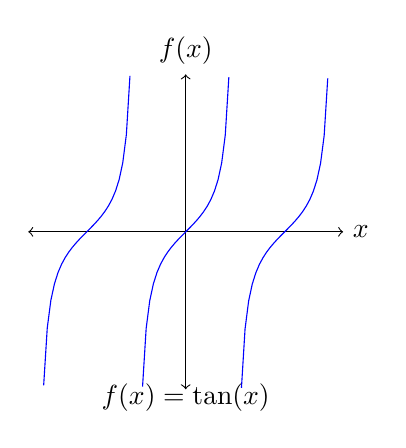
\begin{tikzpicture}[scale=0.4]
        \draw[<->] (-5,0) -- (5,0) node[right] {$x$};
        \draw[<->] (0,-5) -- (0,5) node[above] {$f(x)$};
        \draw[scale=1,domain=-1.37:1.37,variable=\x,blue] plot ({\x},{tan(\x r)});
        \draw[scale=1,domain=1.77:4.51,variable=\x,blue] plot ({\x},{tan(\x r)});
        \draw[scale=1,domain=-4.51:-1.77,variable=\x,blue] plot ({\x},{tan(\x r)});
        \draw (0,-5.25) node {$f(x)=\tan(x)$};
    \end{tikzpicture}\hspace{\stretch{1}}
\end{figure}

\begin{figure}[!ht]
    \centering
    \hspace{\stretch{1}}
    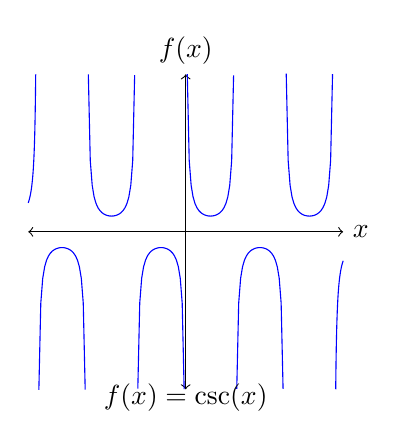
\begin{tikzpicture}[scale=0.2]
        \draw[<->] (-10,0) -- (10,0) node[right] {$x$};
        \draw[<->] (0,-10) -- (0,10) node[above] {$f(x)$};
        \draw[blue,domain=0.1:3.041,variable=\x] plot({\x},{1/(sin(\x r))});
        \draw[blue,domain=-3.041:-0.1,variable=\x] plot({\x},{1/(sin(\x r))});
        \draw[blue,domain=3.242:6.183,variable=\x] plot({\x},{1/(sin(\x r))});
        \draw[blue,domain=-6.183:-3.242,variable=\x] plot({\x},{1/(sin(\x r))});
        \draw[blue,domain=6.383:9.325,variable=\x] plot({\x},{1/(sin(\x r))});
        \draw[blue,domain=-9.325:-6.383,variable=\x] plot({\x},{1/(sin(\x r))});
        \draw[blue,domain=9.525:10,variable=\x] plot({\x},{1/(sin(\x r))});
        \draw[blue,domain=-10:-9.525,variable=\x] plot({\x},{1/(sin(\x r))});
        \draw (0,-10.5) node {$f(x)=\csc(x)$};
    \end{tikzpicture}\hspace{\stretch{1}}
    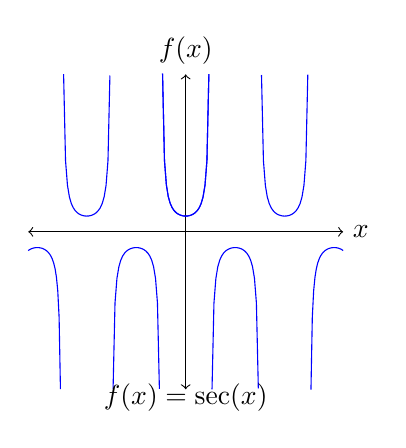
\begin{tikzpicture}[scale=0.2]
        \draw[<->] (-10,0) -- (10,0) node[right] {$x$};
        \draw[<->] (0,-10) -- (0,10) node[above] {$f(x)$};
        \draw[blue,domain=-1.471:1.471,variable=\x] plot({\x},{1/(cos(\x r))});
        \draw[blue,domain=4.813:7.754,variable=\x] plot({\x},{1/(cos(\x r))});
        \draw[blue,domain=-7.754:-4.813,variable=\x] plot({\x},{1/(cos(\x r))});
        \draw[blue,domain=-1.471:1.471,variable=\x] plot({\x},{1/(cos(\x r))});
        \draw[blue,domain=1.671:4.612,variable=\x] plot({\x},{1/(cos(\x r))});
        \draw[blue,domain=-4.612:-1.671,variable=\x] plot({\x},{1/(cos(\x r))});
        \draw[blue,domain=-10:-7.954,variable=\x] plot({\x},{1/(cos(\x r))});
        \draw[blue,domain=7.954:10,variable=\x] plot({\x},{1/(cos(\x r))});
        \draw (0,-10.5) node {$f(x)=\sec(x)$};
    \end{tikzpicture}\hspace{\stretch{1}}
    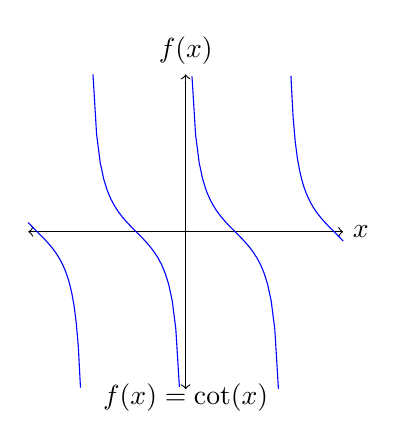
\begin{tikzpicture}[scale=0.4]
        \draw[<->] (-5,0) -- (5,0) node[right] {$x$};
        \draw[<->] (0,-5) -- (0,5) node[above] {$f(x)$};
        \draw[scale=1,domain=3.341:5,variable=\x,blue] plot ({\x},{1/(tan(\x r))});
        \draw[scale=1,domain=-2.944:-0.2,variable=\x,blue] plot ({\x},{1/(tan(\x r))});
        \draw[scale=1,domain=0.2:2.944,variable=\x,blue] plot ({\x},{1/(tan(\x r))});
        \draw[scale=1,domain=-5:-3.341,variable=\x,blue] plot ({\x},{1/(tan(\x r))});
        \draw (0,-5.25) node {$f(x)=\cot(x)$};
    \end{tikzpicture}\hspace{\stretch{1}}
\end{figure}

\begin{figure}[!ht]
    \centering
    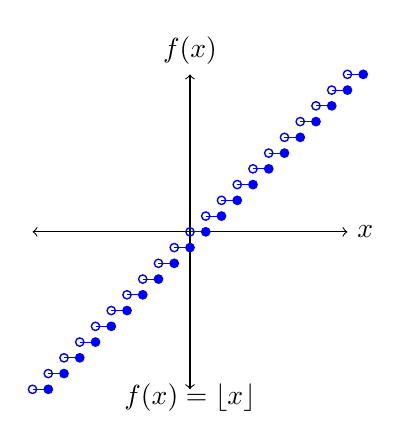
\begin{tikzpicture}[scale=0.20]
    \tkzInit[xmin = -10, xmax = 10, ymin = -10, ymax = 10]
        \draw[<->] (-10,0) -- (10,0) node[right] {$x$};
        \draw[<->] (0,-10) -- (0,10) node[above] {$f(x)$};
    \foreach \a in {-10,...,10}{
        \draw[blue] (\a, \a) -- (\a + 1, \a);
        \node [circle, draw, fill=none, line width = .5pt, color = blue, inner sep = 0pt, minimum size = 3pt] (ca) at (\a, \a) {};
        \node [circle, draw, fill, line width = .5pt, color = blue, inner sep = 0pt, minimum size = 3pt] (ca) at (\a + 1, \a) {};
    }
    \draw (0,-10.5) node {$f(x)=\lfloor{x}\rfloor$};
    \end{tikzpicture}
    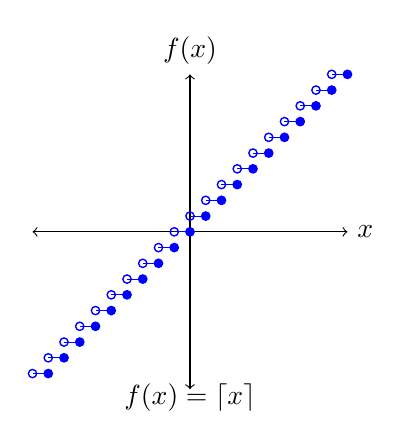
\begin{tikzpicture}[scale=0.20]
    \tkzInit[xmin = -10, xmax = 10, ymin = -10, ymax = 10]
        \draw[<->] (-10,0) -- (10,0) node[right] {$x$};
        \draw[<->] (0,-10) -- (0,10) node[above] {$f(x)$};
    \foreach \a in {-9,...,10}{
        \draw[blue] (\a - 1, \a) -- (\a, \a);
        \node [circle, draw, fill=none, line width = .5pt, color = blue, inner sep = 0pt, minimum size = 3pt] (ca) at (\a-1, \a) {};
        \node [circle, draw, fill, line width = .5pt, color = blue, inner sep = 0pt, minimum size = 3pt] (ca) at (\a, \a) {};
    }
    \draw (0,-10.5) node {$f(x)=\lceil{x}\rceil$};
    \end{tikzpicture}
    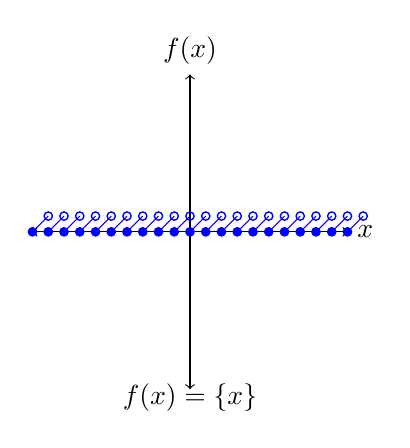
\begin{tikzpicture}[scale=0.20]
    \tkzInit[xmin = -10, xmax = 10, ymin = -10, ymax = 10]
        \draw[<->] (-10,0) -- (10,0) node[right] {$x$};
        \draw[<->] (0,-10) -- (0,10) node[above] {$f(x)$};
    \foreach \a in {-10,...,10}{
        \draw[blue] (\a, 0) -- (\a + 1, 1);
        \node [circle, draw, fill, line width = .5pt, color = blue, inner sep = 0pt, minimum size = 3pt] (ca) at (\a, 0) {};
        \node [circle, draw, fill=none, line width = .5pt, color = blue, inner sep = 0pt, minimum size = 3pt] (ca) at (\a + 1, 1) {};
    }
    \draw (0,-10.5) node {$f(x)=\{x\}$};
    \end{tikzpicture}
\end{figure}
\end{document}